\chapter{Metrik Uzaylar}

Metrik uzaylar, mesafe fonksiyonuna dayanan topolojik yapılardır. Her metrik uzay
doğal olarak bir topolojik uzay oluşturur; bu yapı ``indüklenen topoloji'' olarak adlandırılır.

%-------------------------------------------------------------------
\section{Konu}

\subsection{Sezgisel Giriş — ``Mesafe Topolojiyi Doğurur''}

Metrik uzayı tek cümlede özetlemek gerekirse: \emph{noktalar arasındaki mesafe
fikrinden bir topoloji üretmektir.} Elimizde yalnız ``iki nokta ne kadar uzak?''
sorusunu yanıtlayan bir $d(x,y)$ fonksiyonu vardır; bundan ``bir noktanın yakınında
olmak'' kavramını --- yani açık kümeleri --- kurarız. Köprü tek bir nesnedir:
\textbf{açık yuvar.}

\begin{figure}[ht]
  \centering
  \begin{tikzpicture}[font=\small, etiket/.style={font=\scriptsize}]
  % --- Acik yuvar B(x,r): merkez x, yaricap r, kesikli sinir (sinir dahil degil) ---
  \def\R{2.4}
  % yuvar ici
  \fill[blue!12] (0,0) circle (\R);
  % kesikli cember: sinir B(x,r)'ye dahil DEGIL
  \draw[blue!70!black, very thick, dashed] (0,0) circle (\R);
  % merkez
  \fill[black] (0,0) circle (1.6pt);
  \node[below left=1pt] at (0,0) {$x$};
  % yaricap oku
  \draw[-{Stealth[length=2.4mm]}, thick] (0,0) -- (35:\R)
    node[midway, above, sloped, etiket] {$r$};
  % ic nokta y (dahil)
  \fill[teal!70!black] (-1.0,0.7) circle (1.6pt);
  \node[teal!60!black, etiket, below=1pt] at (-1.0,0.7) {$y$};
  \node[teal!60!black, etiket, align=center] at (-1.05,1.35) {$d(x,y)<r$\\(dahil)};
  % dis nokta z (haric)
  \fill[red!70!black] (62:3.05) circle (1.6pt);
  \node[red!60!black, etiket, right=1pt] at (62:3.05) {$z$};
  \node[red!60!black, etiket, align=center] at (3.0,2.65) {$d(x,z)\ge r$\\(haric)};

  \node[etiket, align=center, fill=blue!6, rounded corners, inner sep=4pt]
    at (0,-3.15)
    {$B(x,r)=\{y\in M : d(x,y)<r\}$ --- kesikli sınır açık yuvara \textbf{dahil değildir}.};
\end{tikzpicture}

  \caption{Açık yuvar $B(x,r)$: merkez $x$'ten $r$'den daha yakın olan tüm
    noktalar; kesikli sınır yuvara dahil değildir.}
\end{figure}

Bu yuvarları temel taş yaparak indüklenen topolojiyi kurarız: bir küme açıktır
$\Leftrightarrow$ her noktasının etrafına tümüyle içeride kalan bir açık yuvar sığar.

\begin{sezgi}
Metrik, sayısal bir ``uzaklık cetveli''dir; topoloji ise yalnız ``yakın mı, uzak
mı?'' sorusunu önemser. Aynı topolojiyi farklı cetveller (metrikler) üretebilir ---
önemli olan hangi noktaların hangi yuvarın \emph{içinde} kaldığıdır, mesafenin tam
sayısal değeri değil.
\end{sezgi}

Aynı düzlem üzerinde farklı metrikler farklı biçimde yuvarlar üretir ama çoğu zaman
\textbf{aynı topolojiyi} indükler:

\begin{figure}[ht]
  \centering
  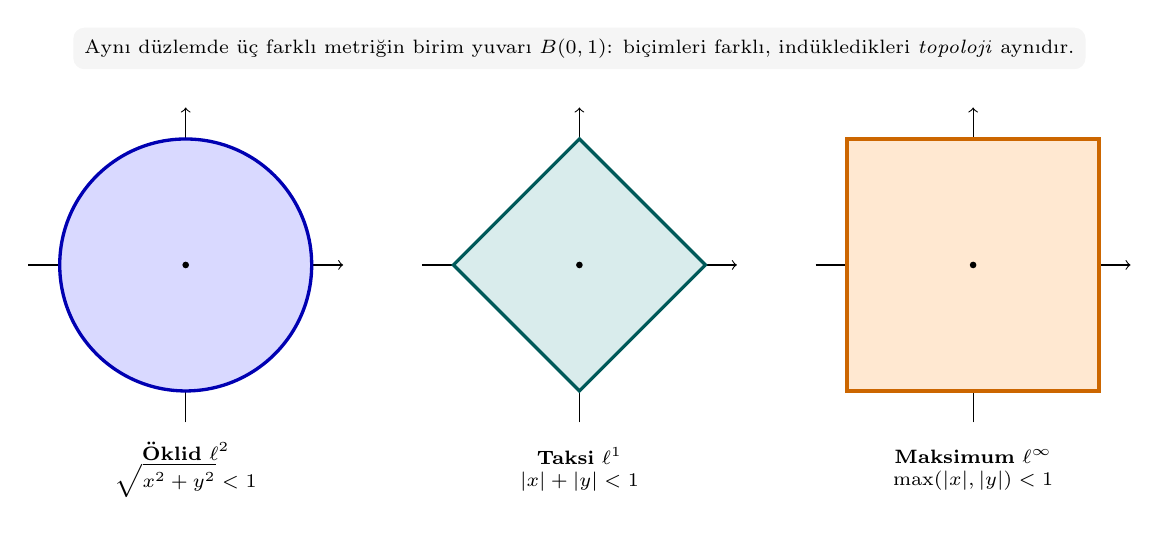
\begin{tikzpicture}[font=\small, etiket/.style={font=\scriptsize}]
  % --- Uc metrigin birim yuvari B(0,1) ---
  \def\S{1.6}  % olcek

  % ---- 1) Oklid metrigi: cember ----
  \begin{scope}[shift={(0,0)}]
    \draw[->] (-\S-0.4,0) -- (\S+0.4,0);
    \draw[->] (0,-\S-0.4) -- (0,\S+0.4);
    \fill[blue!15] (0,0) circle (\S);
    \draw[blue!70!black, very thick] (0,0) circle (\S);
    \fill[black] (0,0) circle (1.2pt);
    \node[etiket, align=center] at (0,-\S-1.0)
      {\textbf{Öklid} $\ell^2$\\$\sqrt{x^2+y^2}<1$};
  \end{scope}

  % ---- 2) Taksi (Manhattan) metrigi: elmas / kare ----
  \begin{scope}[shift={(2*\S+1.8,0)}]
    \draw[->] (-\S-0.4,0) -- (\S+0.4,0);
    \draw[->] (0,-\S-0.4) -- (0,\S+0.4);
    \fill[teal!15] (\S,0) -- (0,\S) -- (-\S,0) -- (0,-\S) -- cycle;
    \draw[teal!70!black, very thick] (\S,0) -- (0,\S) -- (-\S,0) -- (0,-\S) -- cycle;
    \fill[black] (0,0) circle (1.2pt);
    \node[etiket, align=center] at (0,-\S-1.0)
      {\textbf{Taksi} $\ell^1$\\$|x|+|y|<1$};
  \end{scope}

  % ---- 3) Maksimum (Cebysev) metrigi: eksen-hizali kare ----
  \begin{scope}[shift={(4*\S+3.6,0)}]
    \draw[->] (-\S-0.4,0) -- (\S+0.4,0);
    \draw[->] (0,-\S-0.4) -- (0,\S+0.4);
    \fill[orange!18] (-\S,-\S) rectangle (\S,\S);
    \draw[orange!80!black, very thick] (-\S,-\S) rectangle (\S,\S);
    \fill[black] (0,0) circle (1.2pt);
    \node[etiket, align=center] at (0,-\S-1.0)
      {\textbf{Maksimum} $\ell^\infty$\\$\max(|x|,|y|)<1$};
  \end{scope}

  \node[etiket, align=center, fill=gray!8, rounded corners, inner sep=4pt]
    at (2*\S+1.8,\S+1.15)
    {Aynı düzlemde üç farklı metriğin birim yuvarı $B(0,1)$:
     biçimleri farklı, indükledikleri \emph{topoloji} aynıdır.};
\end{tikzpicture}

  \caption{Üç farklı metriğin birim yuvarı $B(0,1)$: Öklid çember, taksi
    (Manhattan) elması, maksimum metrik karesi --- biçimleri farklı, indükledikleri
    topoloji aynı.}
\end{figure}

\subsection{Metrik Aksiyomları}

\begin{definition}[Metrik Uzay]
$M$ kümesi ve $d: M \times M \to [0,\infty)$ verilsin.
$(M, d)$ bir \textbf{metrik uzay}, $d$ ise \textbf{metrik} ise:
\begin{enumerate}
  \item[(M1)] \textbf{Özdeşlik:} $d(x,y) = 0 \Leftrightarrow x = y$
  \item[(M2)] \textbf{Simetri:} $d(x,y) = d(y,x)$
  \item[(M3)] \textbf{Üçgen:} $d(x,z) \leq d(x,y) + d(y,z)$
\end{enumerate}
\end{definition}

Üçgen eşitsizliği, üç aksiyom içinde en derin olanıdır: ``$x$'ten $z$'ye doğrudan
gitmek, $y$'ye uğrayıp gitmekten kısadır'' der.

\begin{figure}[ht]
  \centering
  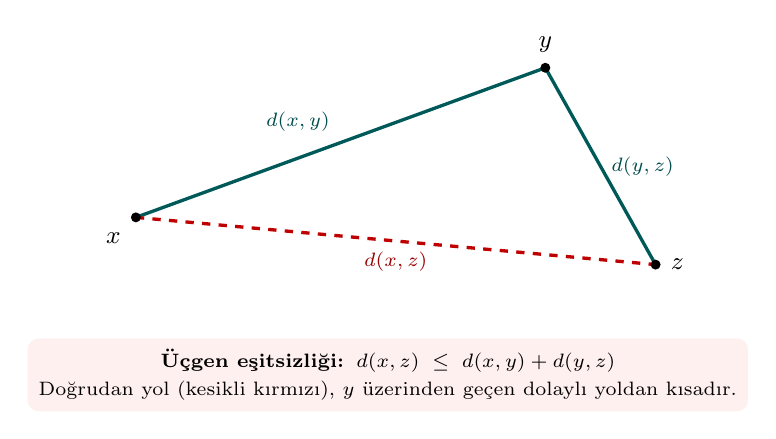
\begin{tikzpicture}[font=\small, etiket/.style={font=\scriptsize}]
  % --- Ucgen esitsizligi: d(x,z) <= d(x,y) + d(y,z) ---
  \coordinate (x) at (0,0);
  \coordinate (y) at (5.2,1.9);
  \coordinate (z) at (6.6,-0.6);

  % dolayli yol x -> y -> z
  \draw[teal!70!black, very thick] (x) -- (y)
    node[midway, above left, etiket, teal!60!black] {$d(x,y)$};
  \draw[teal!70!black, very thick] (y) -- (z)
    node[midway, right, etiket, teal!60!black] {$d(y,z)$};
  % dogrudan yol x -> z (kestirme)
  \draw[red!75!black, very thick, dashed] (x) -- (z)
    node[midway, below, etiket, red!60!black] {$d(x,z)$};

  % noktalar
  \foreach \p/\pos in {x/{below left}, y/{above}, z/{right}} {
    \fill[black] (\p) circle (1.8pt);
    \node[\pos=2pt] at (\p) {$\p$};
  }

  \node[etiket, align=center, fill=red!6, rounded corners, inner sep=4pt]
    at (3.2,-2.0)
    {\textbf{Üçgen eşitsizliği:}\;\;$d(x,z)\;\le\;d(x,y)+d(y,z)$\\[2pt]
     Doğrudan yol (kesikli kırmızı), $y$ üzerinden geçen dolaylı yoldan kısadır.};
\end{tikzpicture}

  \caption{Üçgen eşitsizliği: $x$'ten $z$'ye doğrudan mesafe, $y$ üzerinden geçen
    dolaylı yoldan kısadır.}
\end{figure}

\begin{karsiornek}
\textbf{Üçgen eşitsizliği şart.} $\{A,B,C\}$ üzerinde $d(A,B)=1$, $d(B,C)=1$ ama
$d(A,C)=5$ koyalım (özdeşlik ve simetri korunsun). M1 ve M2 sağlanır, ama
$d(A,C)=5 > d(A,B)+d(B,C)=2$ olduğundan M3 ihlal edilir. Bu fonksiyon bir
\emph{metrik değildir}; ürettiği ``yuvarlar'' tutarlı bir topoloji vermez.
\texttt{validate\_metric} bu durumu yakalar (Alıştırma K4).
\end{karsiornek}

\subsection{Temel Kavramlar}

\begin{itemize}
  \item \textbf{Açık top:} $B(x, r) = \{y \in M : d(x,y) < r\}$
  \item \textbf{Kapalı top:} $\bar{B}(x, r) = \{y \in M : d(x,y) \leq r\}$
  \item \textbf{İndüklenen topoloji:} $\tau_d = \{U : \forall x \in U,\,\exists\varepsilon>0,\,B(x,\varepsilon) \subseteq U\}$
  \item \textbf{Çap:} $\mathrm{diam}(A) = \sup\{d(x,y) : x,y \in A\}$
\end{itemize}

\subsection{Standart Metrikler}

\begin{table}[h]
\centering
\begin{tabular}{lll}
\toprule
\textbf{Metrik} & \textbf{Tanım} & \textbf{Uzay} \\
\midrule
Öklid & $d(x,y) = |x-y|$ & $\mathbb{R}$ \\
Ayrık & $d(x,y) = 0$ veya $1$ & Herhangi $X$ \\
$\ell^\infty$ (max) & $\max_i d_i(x_i,y_i)$ & Çarpım uzayı \\
Sınırlı (capped) & $d'(x,y) = \min(d(x,y),1)$ & Eşdeğer topoloji \\
\bottomrule
\end{tabular}
\caption{Standart metrikler}
\end{table}

%-------------------------------------------------------------------
\section{Teoremler}

\begin{theorem}
Her metrik uzay Hausdorff (T2) ve $1^{\text{st}}$ sayılabilirdir.
\end{theorem}

\begin{proof}[İspat eskizi]
(T2) $x \neq y$ olsun; o hâlde $r = d(x,y) > 0$ (M1). $B(x, r/2)$ ve $B(y, r/2)$
yuvarları ayrıktır: ortak bir $z$ noktası olsaydı, üçgen eşitsizliğinden (M3)
$r = d(x,y) \leq d(x,z) + d(z,y) < r/2 + r/2 = r$ çelişkisi çıkardı. Demek ki $x$ ve
$y$ açık komşuluklarla ayrılır. (1.\ sayılabilir) Her $x$ için sayılabilir
$\{B(x, 1/n) : n \in \mathbb{N}\}$ ailesi yerel bazdır: $x \in U$ açık ise
$B(x,\varepsilon) \subseteq U$ olacak $\varepsilon > 0$ vardır; $1/n < \varepsilon$
seçince $B(x, 1/n) \subseteq U$.
\end{proof}

\begin{theorem}[Sınırlı Metrik Eşdeğerliği]
$d'(x,y) = \min(d(x,y),1)$ ile $d$ aynı topolojiyi indükler.
\end{theorem}

\begin{proof}[İspat eskizi]
İki metrik aynı topolojiyi indükler $\Leftrightarrow$ her $d$-açık yuvarın içine bir
$d'$-açık yuvar sığar ve tersi. Yarıçapı $r \leq 1$ olan yuvarlarda
$B_d(x, r) = B_{d'}(x, r)$ tam çakışır, çünkü $d$ ile $d'$ yalnız mesafesi $\geq 1$
olan çiftlerde ayrışır. Topoloji ``yeterince küçük yuvarlar'' tarafından
belirlendiğinden büyük yarıçaplı farklılık topolojiyi değiştirmez; $\tau_d = \tau_{d'}$.
\end{proof}

\begin{theorem}
$\mathbb{R}^n$ üzerindeki max, sum ve Öklid metrikleri topolojik olarak eşdeğerdir.
\end{theorem}

\begin{proof}[İspat eskizi]
Üç metrik karşılıklı sabit çarpanlarla sınırlanır:
$d_\infty \leq d_2 \leq d_1 \leq n\,d_\infty$ (max $\leq$ Öklid $\leq$ taksi
$\leq n\cdot$max). Böyle bir ``sandviç'' her metriğin yuvarının içine ötekinin
yuvarını sığdırır (ör.\ $B_\infty(x, r/n) \subseteq B_1(x, r) \subseteq B_\infty(x, r)$).
Karşılıklı içerme $\Rightarrow$ aynı açık kümeler $\Rightarrow$ aynı topoloji.
Bölüm 1.0'daki birim-yuvar figürü bu üç biçimi yan yana gösterir.
\end{proof}

%-------------------------------------------------------------------
\section{Algoritmalar}

\subsection{validate\_metric — $O(|X|^3)$}

\begin{algorithm}
\caption{ValidateMetric$(X, d)$}
\begin{algorithmic}[1]
\For{each $x \in X$}
    \If{$d(x,x) \neq 0$} \Return False \EndIf
    \For{each $y \neq x$}
        \If{$d(x,y) = 0$} \Return False \EndIf
    \EndFor
\EndFor
\For{each $x,y \in X$}
    \If{$d(x,y) \neq d(y,x)$} \Return False \EndIf
\EndFor
\For{each $x,y,z \in X$}
    \If{$d(x,z) > d(x,y) + d(y,z)$} \Return False \EndIf
\EndFor
\State \Return True
\end{algorithmic}
\end{algorithm}

Karmaşıklık: $O(|X|^3)$ — üçgen eşitsizliği dominates.

\subsection{open\_ball — $O(|X|)$}

\begin{algorithm}
\caption{OpenBall$(x, r, X, d)$}
\begin{algorithmic}[1]
\State \Return $\{y \in X : d(x,y) < r\}$
\end{algorithmic}
\end{algorithm}

%-------------------------------------------------------------------
\section{pytop API}

\begin{lstlisting}[language=Python]
from pytop.metric_spaces import (
    FiniteMetricSpace,
    SymbolicMetricSpace,
    validate_metric,
)
from pytop import (
    open_ball,
    closed_ball,
    distance_to_subset,
    diameter_of_subset,
    is_bounded_subset,
    capped_metric,
)
\end{lstlisting}

\texttt{FiniteMetricSpace(carrier=tuple, distance=dict)} — mesafe sözlüğü \texttt{(a,b): float}.

\texttt{open\_ball(fms, point, radius)} $\to$ \texttt{set} döner (Result değil).

\texttt{capped\_metric(distance\_fn, cap=1.0)} $\to$ \texttt{Callable} döner.

\textbf{Metrik $\to$ TDA köprüsü:} Bir \texttt{FiniteMetricSpace}
(\texttt{carrier} + \texttt{distance}) doğrudan
\texttt{pytop.persistent\_homology(space, max\_dimension=, max\_scale=)} fonksiyonuna
beslenebilir; bu, ham nokta bulutunu Vietoris–Rips filtrasyonuna çevirip kalıcı
homolojiyi hesaplar. Dönen \texttt{PersistencePair} alanları: \texttt{dimension},
\texttt{birth}, \texttt{death}, \texttt{persistence}, \texttt{is\_essential}
(Örnek 5.8).

%-------------------------------------------------------------------
\section{Örnekler}

\subsection*{Örnek 5.1 — Ayrık Metrik Uzay}

\begin{lstlisting}[language=Python]
points = [1, 2, 3, 4]
dist_discrete = {(a, b): (0 if a == b else 1)
                 for a in points for b in points}
fms = FiniteMetricSpace(carrier=tuple(points), distance=dist_discrete)
print("carrier:", fms.carrier)
print("d(1,2):", fms.distance[(1,2)])
\end{lstlisting}

\begin{verbatim}
carrier: (1, 2, 3, 4)
d(1,2): 1
\end{verbatim}

\subsection*{Örnek 5.3 — open\_ball}

\begin{lstlisting}[language=Python]
print("B(1, 0.5) =", open_ball(fms, 1, 0.5))
print("B(1, 1.5) =", open_ball(fms, 1, 1.5))
\end{lstlisting}

\begin{verbatim}
B(1, 0.5) = {1}
B(1, 1.5) = {1, 2, 3, 4}
\end{verbatim}

\subsection*{Örnek 5.6 — capped\_metric}

\begin{lstlisting}[language=Python]
cap_fn = capped_metric(fms_line.distance, cap=1.0)
print("d(0,3) capped:", cap_fn(0, 3))
print("d(0,1) capped:", cap_fn(0, 1))
\end{lstlisting}

\begin{verbatim}
d(0,3) capped: 1.0
d(0,1) capped: 1.0
\end{verbatim}

\subsection*{Örnek 5.7 — Üç Metrik, Üç Yuvar, Aynı Geçerlilik}

Düzlemdeki aynı beş nokta üzerinde Öklid, taksi ($\ell^1$) ve maksimum
($\ell^\infty$) metriklerini kurarız: üçü de geçerli metriktir ama aynı çift için
farklı mesafe verir (Bölüm 1.0 birim-yuvar figürünün sayısal karşılığı).

\begin{lstlisting}[language=Python]
import math
from pytop.metric_spaces import FiniteMetricSpace, validate_metric

grid = [(0, 0), (1, 0), (0, 1), (1, 1), (2, 1)]
carrier = tuple(range(len(grid)))

def euclid(i, j):    return math.dist(grid[i], grid[j])
def taxicab(i, j):   return abs(grid[i][0]-grid[j][0]) + abs(grid[i][1]-grid[j][1])
def chebyshev(i, j): return max(abs(grid[i][0]-grid[j][0]), abs(grid[i][1]-grid[j][1]))

for name, d in [("Oklid", euclid), ("Taksi", taxicab), ("Maksimum", chebyshev)]:
    dist = {(i, j): d(i, j) for i in carrier for j in carrier}
    fms = FiniteMetricSpace(carrier=carrier, distance=dist)
    print(name, "d(0,4)=", round(dist[(0,4)], 4), "metrik?", validate_metric(fms).status)
\end{lstlisting}

\begin{verbatim}
Oklid    d(0,4)= 2.2361 metrik? true
Taksi    d(0,4)= 3.0    metrik? true
Maksimum d(0,4)= 2.0    metrik? true
\end{verbatim}

Mesafeler farklı (Öklid $\sqrt5$, taksi $3$, maksimum $2$), ama üçü de aynı
topolojiyi indükler (Teorem 2.3).

\subsection*{Örnek 5.8 — Metrik $\to$ Kalıcı Homoloji (TDA Köprüsü)}

Metrik uzayın hesaplama gücüne köprü: bir nokta bulutundan \texttt{FiniteMetricSpace}
kurup doğrudan \texttt{persistent\_homology}'ye veririz. Çember üzerinde örneklenmiş
8 nokta --- ``delik'' (1-boyutlu döngü) topolojik imza olarak ortaya çıkmalıdır.

\begin{lstlisting}[language=Python]
import math, pytop
from pytop.metric_spaces import FiniteMetricSpace

n = 8
pts = [(math.cos(2*math.pi*k/n), math.sin(2*math.pi*k/n)) for k in range(n)]
carrier = tuple(range(n))
dist = {(i, j): math.dist(pts[i], pts[j]) for i in carrier for j in carrier}
circle = FiniteMetricSpace(carrier=carrier, distance=dist)

pairs = pytop.persistent_homology(circle, max_dimension=2, max_scale=2.5)
components = [p for p in pairs if p.dimension == 0 and p.is_essential]
loops = [p for p in pairs if p.dimension == 1]
loop = loops[0]
print("bilesen (H0):", len(components), " dongu (H1):", len(loops))
print("dongu: dogum=", round(loop.birth,4), "olum=", round(loop.death,4))
\end{lstlisting}

\begin{verbatim}
bilesen (H0): 1  dongu (H1): 1
dongu: dogum= 0.7654 olum= 1.8478
\end{verbatim}

Tam beklenen sonuç: çember bağlantılı olduğundan tek kalıcı bileşen ($H_0$), bir
deliği olduğundan tek kalıcı döngü ($H_1$). Döngü, komşu noktalar bağlandığında
doğar ($\approx 0.765$) ve yarıçap deliği dolduracak kadar büyüyünce ölür
($\approx 1.848$). Ham koordinatlardan (\texttt{math.dist}) pytop topolojik bir
özelliği --- deliğin varlığını --- sayısal olarak çıkardı.

%-------------------------------------------------------------------
\section{Alıştırmalar}

\subsection*{Kodlama}

\begin{enumerate}[label=K\arabic*.]
\item $\{A,B,C,D\}$ üzerinde bir metrik tanımlayın ve \texttt{validate\_metric} ile
      doğrulayın. Üçgen eşitsizliğini ihlal eden bir örnek de deneyin.
\item Öklid metrikli $\{0,\ldots,9\}$ üzerinde $B(5,3.0)$ ve $\bar{B}(5,3.0)$
      hesaplayın.
\item \texttt{normalized\_metric} kullanarak bir metriği $[0,1]$'e normalleştirin.
\item \S 1.0'daki karşı-örneği koda dökün: $\{A,B,C,D\}$ üzerinde $d(A,C)=5$,
      $d(A,B)=d(B,C)=1$ olan bir mesafe sözlüğü kurun (geri kalanını ayrık metrikle
      doldurun) ve \texttt{validate\_metric} ile üçgen eşitsizliğinin ihlal
      edildiğini gösterin; \texttt{justification} alanını yazdırın.
\item \emph{(TDA köprüsü)} Birim kareyi örnekleyen \textbf{dolu} bir $3\times 3$
      ızgara (9 nokta) üzerinde Öklid \texttt{FiniteMetricSpace} kurun ve
      \texttt{persistent\_homology(space, max\_dimension=2, max\_scale=2.5)}
      çalıştırın. $H_1$ döngülerinin \texttt{persistence} değerlerine bakın:
      Örnek 5.8'deki çemberin uzun ömürlü ($\approx 1.08$) döngüsüne benzer
      \textbf{kalıcı} bir döngü var mı? Dolu karenin neden gerçek bir deliği yoktur?
\end{enumerate}

\subsection*{Teori}

\begin{enumerate}[label=T\arabic*.]
\item Her metrik uzayın Hausdorff olduğunu ispatlayın.
\item $d' = \min(d,1)$ ve $d$ aynı topolojiyi indüklediğini gösterin.
\item Üçgen eşitsizliğinin (M3) Teorem 2.1'deki Hausdorff ispatında tam olarak
      nerede kullanıldığını açıklayın. (İpucu: $B(x, r/2)$ ve $B(y, r/2)$'nin ayrık
      olduğunu gösteren adım hangisidir?)
\end{enumerate}
